\documentclass[a4paper,10pt]{article}
\usepackage{luatexja}
\usepackage{luatexja-fontspec}
\usepackage{geometry}
\usepackage{multicol}
\usepackage{titlesec}
\usepackage{setspace}
\usepackage{graphicx}
\usepackage{caption}
\usepackage{indentfirst}
\usepackage{float} % 図の位置を制御するために追加
\usepackage{listings}
\usepackage{xcolor}
\usepackage{amsmath} % align 環境などの数式用
\usepackage{hyperref}

\geometry{margin=20mm}
\setstretch{1.2}
\parindent=1em

% ===== 日本語フォント設定 =====
% HaranoAjiMincho がシステムに入っている必要あり
\setmainjfont{HaranoAjiMincho} % メイン日本語フォント
\setsansjfont{HaranoAjiGothic} % サンセリフ（任意）
\setmonojfont{HaranoAjiMincho} % 等幅も同じに設定（好みに応じて変更）

% 図のキャプションの表記を「図1」のように日本語化
\renewcommand{\figurename}{図}
\captionsetup[figure]{labelformat=default,labelsep=period}

\renewcommand{\tablename}{表}
\captionsetup[table]{labelformat=default,labelsep=period}

\geometry{margin=25mm}
\setstretch{1.2}
\parindent=1em

\titleformat{\section}{\large\bfseries}{\thesection.}{1em}{}

\definecolor{keywordcolor}{rgb}{0.26, 0.38, 0.68}
\definecolor{commentcolor}{rgb}{0.3, 0.6, 0.3}
\definecolor{stringcolor}{rgb}{0.7, 0.2, 0.2}

\lstdefinelanguage{SystemVerilog}{
  morekeywords={module,endmodule,input,output,logic,always_ff,if,else,begin,end,posedge,negedge},
  sensitive=true,
  morecomment=[l]{//},
  morecomment=[s]{/*}{*/},
  morestring=[b]",
}

\lstset{
  language=SystemVerilog,
  basicstyle=\ttfamily\small,
  keywordstyle=\color{keywordcolor}\bfseries,
  commentstyle=\color{commentcolor}\itshape,
  stringstyle=\color{stringcolor},
  numbers=left,
  numberstyle=\tiny,
  stepnumber=1,
  numbersep=5pt,
  frame=single,
  tabsize=2,
  showstringspaces=false,
  breaklines=true,
  breakatwhitespace=true
}

% -------------------------------------------
% Python 用の listings 言語定義
% -------------------------------------------
\lstdefinelanguage{PythonCustom}{
  language=Python,
  morekeywords={
    def,class,return,import,from,as,with,for,while,if,elif,else,
    try,except,finally,raise,pass,break,continue,lambda,yield,global,nonlocal
  },
  sensitive=true,
  morecomment=[l]{\#},
  morestring=[b]",
}

% -------------------------------------------
% Python 用スタイル
% （SystemVerilog のスタイルを完全踏襲）
% -------------------------------------------
\lstdefinestyle{pythonstyle}{
  language=PythonCustom,
  basicstyle=\ttfamily\small,
  keywordstyle=\color{keywordcolor}\bfseries,
  commentstyle=\color{commentcolor}\itshape,
  stringstyle=\color{stringcolor},
  numbers=left,
  numberstyle=\tiny,
  stepnumber=1,
  numbersep=5pt,
  frame=single,
  tabsize=2,
  showstringspaces=false,
  breaklines=true,
  breakatwhitespace=true
}

% \title{SystemVerilog Code with Listings}

\begin{document}

% タイトルブロック
\begin{center}
\noindent
{\LARGE 第6回輪講資料} \\
{\large 4321　野秋 琳太郎} \\
2026年 1月 22日
\end{center}

\begin{flushright}
指導教員　宮田 尚起
\end{flushright}    

% 二段組開始
\begin{multicols}{2}[\raggedcolumns]
\section{はじめに}
今回は.前々回に導出したKdV方程式を数値計算で解いて.波のふるまいを調べる.
ソリトン解が得られると嬉しい.

\section{卒研の構想}
超高周波回路において.受動素子の非線形性が引き起こすPIM (Passive Intermodulation) は通信品質を劣化させる要因であり.これの強さを評価したい.
具体的な研究手順は以下の通りである.

\begin{enumerate}
    \item \textbf{バラクタダイオードによるモデルの導出} \\
    　まず.非線形特性が理論的に明確な「バラクタダイオード」を用いたLCラダー回路を対象とする.
    キルヒホッフの法則に基づく回路方程式に対し.近似と摂動展開を行うことで.
    非線形波動を記述するKdV (Korteweg-de Vries) 方程式を導出し.そのソリトン解を解析的に求める.

    \item \textbf{MLCCによるモデルの拡張} \\
    　次に.非線形素子を「積層セラミックコンデンサ (MLCC)」に置き換えたモデルを検討する.
    バラクタダイオードによる理想的なソリトン伝搬を基準とし.MLCC特有の非線形性が.ソリトンの波形にどのような差異をもたらすかを比較・分析する.

    \item \textbf{非線形性の逆算} \\
    　KdV方程式において.ソリトンの速度や振幅は.拡散項と非線形項のバランスによって決定される.
    この関係性を利用し.実測で得られたソリトン波形から.逆に素子の非線形パラメータを推定する手法を確立し.MLCCの動的特性の評価を行う.
\end{enumerate}

\section{KdV方程式の導出(前々回の内容)}
\subsection{KdV方程式とは} 
KdV方程式は,非線形波動方程式の一種であり,浅水波やプラズマ波動などの現象を記述するために用いられる. 
その一般的な形は式\ref{eq:kdv}の通りである.
これの解は解析的に求めることができ,図\ref{fig:soliton}に示すようなソリトン波と呼ばれる孤立波を表すことができる.
ここで,式\ref{eq:kdv}の$u(x,t)$を\ref{eq:kdv-solution}として,\ref{eq:kdv-ic}の初期条件を与えている.
この波は,非線形性と分散性のバランスによって形成され,他の波と衝突しても形状を保つ特性を持つ.
例えば,水面に2つの石を別の場所に投げ込んだときに発生する波は,衝突しても元の形状を保ちながら進む.
これはこのソリトン波の特性によるものである.

KdV方程式が非線形波動の中でも広い応用範囲を持つことと,ソリトン波が確認できていることから,
非線形なキャパシタを考慮すれば電信方程式をKdV方程式として解ける形で導出できると考えられる.

\begin{align}
    \frac{\partial u(x,t)}{\partial t} + 6u \frac{\partial u(x,t)}{\partial x} + \frac{\partial^3 u(x,t)}{\partial x^3} = 0 \label{eq:kdv}
\end{align}

\begin{figure}[H]
    \centering
    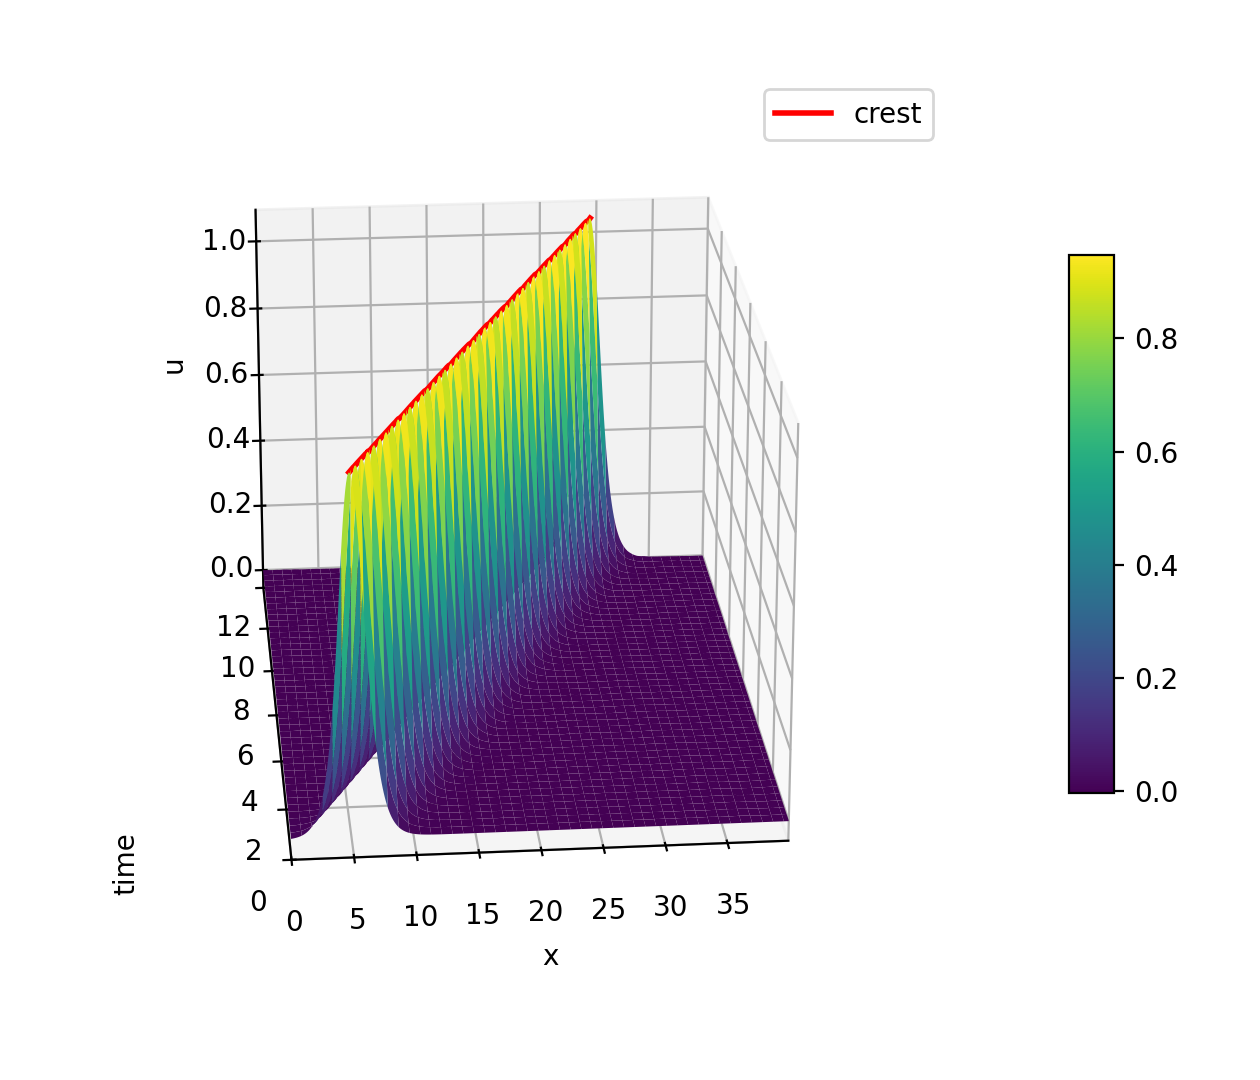
\includegraphics[width=\linewidth]{KdV_surface.png}
    \caption{KdV方程式の孤立波解の例}
    \label{fig:soliton}
\end{figure}

\begin{equation}
  u(x,t)
  = 2k^{2}\,
  \operatorname{sech}^{2}\!\left(
  k\left( x - 4k^{2} t - x_{0} \right)\right)
  \label{eq:kdv-solution}
\end{equation}

\begin{equation}
  u(x,0)
  = \frac{c}{2}\,\operatorname{sech}^2\!\left(
      \frac{\sqrt{c}}{2}\,(x - x_0)
    \right)
  \label{eq:kdv-ic}
\end{equation}

\subsection{非線形キャパシタのモデル}
高周波回路,特に非線形伝送線路の解析において,
キャパシタのモデルとしてバラクタダイオード（Varactor Diode）が重要な役割を果たす.

このキャパシタの静電容量 $C(V)$ は,印加電圧 $V$ に対して非線形な特性を持つ.
この特性を表現するモデルとして,以下の式(\ref{eq:varactor})が広く用いられている.

\begin{equation}
    C(V) = \frac{C_{J0}}{\left( 1 + \frac{V}{\phi} \right)^{\gamma}} \label{eq:varactor}
\end{equation}

ここで,$C_{J0}$ はバイアス電圧がゼロの時の接合容量,$\phi$ は拡散電位（ビルトインポテンシャル）,$\gamma$ は接合容量係数である.
これは物性値で.例えばシリコン階段接合では$\phi = 0.7$.$\gamma = 0.5$ となる.

接合容量$\phi$よりも十分に小さい電圧の信号を印加するものとして,キャパシタの容量$C(V)$ をテイラー展開して1次の項まで近似する.

\begin{equation}
    C(V) \approx C_{J0}\left( 1 - \gamma \frac{V}{\phi} \right) + O(V^2) \label{eq:capacitor_approx}
\end{equation}


\subsection{LCラダーをブシネスク方程式へ}
まず,図\ref{fig:lchasigo}に示すような抵抗 $R$ とコンダクタンス $G$ をゼロに設定した分布定数回路(LCラダー)を考える.
この回路の第 $n$ 番目のノードにおける方程式は, キルヒホッフの法則より以下の差分方程式で記述される.

\begin{figure}[H]
    \centering
    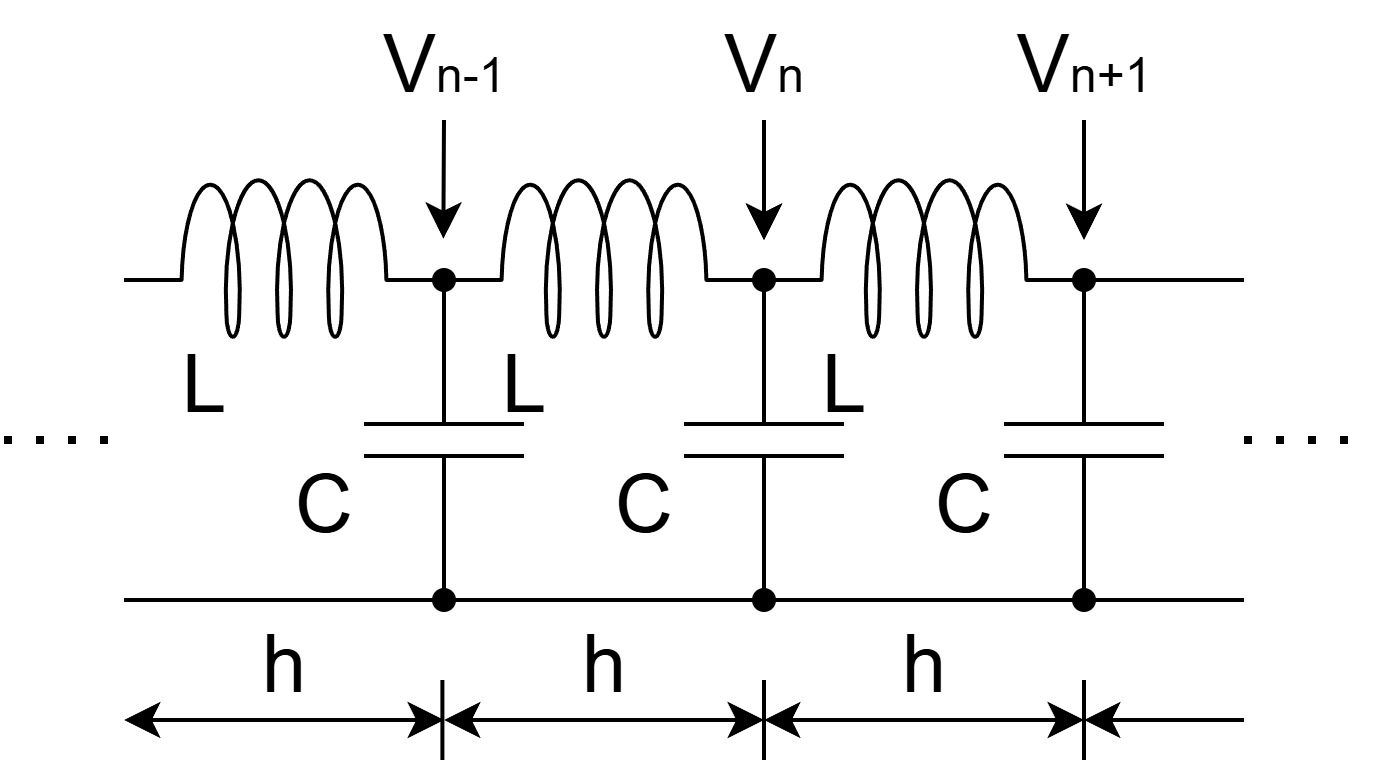
\includegraphics[width=\linewidth]{figure/lchasigo.png}
    \caption{LCラダー回路}
    \label{fig:lchasigo}
\end{figure}

\begin{equation}
    V_{n+1} + V_{n-1} -2V_n= L h^2 \frac{d^2 Q}{dt^2} \label{eq:discrete_wave}
\end{equation}
(※左辺は隣接ノードとの電位差の変化, 右辺は電流の時間変化に対応する)

ここで, 空間的に連続な関数 $V(x, t)$ を仮定し, $V_n(t) = V(x, t)$, $V_{n\pm 1}(t) = V(x \pm h, t)$ と置く.
$V(x \pm h, t)$ を $x$ の周りでテイラー展開すると以下のようになる.

\begin{align}
    &V(x + h) = \notag \\
    &V(x) + h \frac{\partial V}{\partial x} + \frac{h^2}{2!} \frac{\partial^2 V}{\partial x^2} + \frac{h^3}{3!} \frac{\partial^3 V}{\partial x^3} + \frac{h^4}{4!} \frac{\partial^4 V}{\partial x^4} + \cdots \\
    &V(x - h) = \notag\\
    &V(x) - h \frac{\partial V}{\partial x} + \frac{h^2}{2!} \frac{\partial^2 V}{\partial x^2} - \frac{h^3}{3!} \frac{\partial^3 V}{\partial x^3} + \frac{h^4}{4!} \frac{\partial^4 V}{\partial x^4} - \cdots
\end{align}

これら2式の和をとると, 奇数次の項が相殺し, 偶数次の項が残る.
ここで,ターゲットとなるKdV方程式は3次の微分方程式であるため,それが表せる4次の微分項までを残す.

\begin{equation}
    V(x + h) + V(x - h) = 2V(x) + h^2 \frac{\partial^2 V}{\partial x^2} + \frac{h^4}{12} \frac{\partial^4 V}{\partial x^4} + O(h^6)
\end{equation}

これを変形して, 差分方程式の左辺（2階中心差分）に対応させる.

\begin{equation}
    V_{n+1} - 2V_n + V_{n-1} = h^2 \frac{\partial^2 V}{\partial x^2} + \frac{h^4}{12} \frac{\partial^4 V}{\partial x^4} + O(h^6) \label{eq:diff_expansion}
\end{equation}

これまでは $h \to 0$ とし, 第2項以降を無視していたが, ソリトンのような分散性波動を記述する場合, $h$ は有限であるとして第2項（$h^4$ の項）までを考慮する.

式(\ref{eq:diff_expansion})を元の回路方程式(\ref{eq:discrete_wave})に代入する.

\begin{equation}
    h^2 \frac{\partial^2 V}{\partial x^2} + \frac{h^4}{12} \frac{\partial^4 V}{\partial x^4} \approx L h^2 \frac{\partial^2 Q}{\partial t^2}
\end{equation}

両辺を $h^2$ で割り, 整理すると次式が得られる.

\begin{equation}
    \frac{\partial^2 V}{\partial x^2} + \frac{h^2}{12} \frac{\partial^4 V}{\partial x^4} = L \frac{\partial^2 Q}{\partial t^2} \label{eq:wave_basic}
\end{equation}

このように, 離散的な差分を近似する際にテイラー展開の高次項を残すことで, 回路の分散性を表す空間4階微分項 $\frac{\partial^4 V}{\partial x^4}$ が自然に導かれる.

式\ref{eq:capacitor_approx}を電圧 $V$ で積分し, 電荷 $Q(V)$ の近似式を得る.

\begin{equation}
    Q(V) = \int C(V) dV \approx C_{J0} V - \frac{\gamma C_{J0}}{2\phi} V^2 \label{eq:charge_approx}
\end{equation}

式(\ref{eq:charge_approx})を式(\ref{eq:wave_basic})に代入し, 線形位相速度 $v_0 = 1/\sqrt{LC_{J0}}$ を用いて整理すると, 以下の「分散項付き非線形波動方程式（Boussinesq型方程式）」が得られる.
Boussinesq型方程式は, 非線形性と分散性の両方を含む波動現象を記述するために広く知られている.

\begin{equation}
    \frac{1}{v_0^2}\frac{\partial^2 V}{\partial t^2} - \frac{\partial^2 V}{\partial x^2} - \frac{h^2}{12}\frac{\partial^4 V}{\partial x^4} - \frac{\gamma}{2\phi v_0^2}\frac{\partial^2 (V^2)}{\partial t^2} = 0 \label{eq:boussinesq}
\end{equation}

\subsection{Gardner-Morikawa変換でKdV方程式へ}
式(\ref{eq:boussinesq})で与えられたブシネスク方程式から,一方向に伝播する波を記述するKdV方程式を導出する.
導出には,波と共に動く座標系への変換と,微小パラメータ $\epsilon$ を用いた摂動展開（逓減摂動法）を用いる.

まず,空間座標 $x$ と時間 $t$ に対し,以下の独立変数変換を行う.
\begin{equation}
    \xi = x - v_0 t, \quad \tau = \epsilon t
\end{equation}
ここで,$v_0$ は波の位相速度である.この変換により,微分演算子は連鎖律を用いて次のように書き換えられる.
\begin{equation}
    \frac{\partial}{\partial x} = \frac{\partial}{\partial \xi}, \quad
    \frac{\partial}{\partial t} = -v_0 \frac{\partial}{\partial \xi} + \epsilon \frac{\partial}{\partial \tau}
\end{equation}
特に,時間の2階微分については,十分に小さい数である$\epsilon$ の2次以上の項を無視すると,以下の近似式が得られる.
\begin{equation}
    \frac{\partial^2}{\partial t^2} \approx v_0^2 \frac{\partial^2}{\partial \xi^2} - 2v_0 \epsilon \frac{\partial^2}{\partial \xi \partial \tau}
\end{equation}
これらの関係式を元のブシネスク方程式(\ref{eq:boussinesq})の各項に代入する.まず,線形項（第1項と第2項）は次のように整理される.
\begin{align}
    \frac{1}{v_0^2}\frac{\partial^2 V}{\partial t^2} - \frac{\partial^2 V}{\partial x^2} 
    &\approx \frac{1}{v_0^2} \left( v_0^2 \frac{\partial^2 V}{\partial \xi^2} - 2v_0 \epsilon \frac{\partial^2 V}{\partial \xi \partial \tau} \right) - \frac{\partial^2 V}{\partial \xi^2} \notag \\
    &= -\frac{2\epsilon}{v_0} \frac{\partial^2 V}{\partial \xi \partial \tau}
\end{align}
次に,分散項（第3項）と非線形項（第4項）については,$\epsilon$ の最低次の項のみを考慮し,時間微分の主要項 $\partial_t^2 \approx v_0^2 \partial_\xi^2$ を用いることで次のように近似される.
\begin{align}
    \frac{h^2}{12}\frac{\partial^4 V}{\partial x^4} &= \frac{h^2}{12}\frac{\partial^4 V}{\partial \xi^4} \\
    \frac{\gamma}{2\phi v_0^2}\frac{\partial^2 (V^2)}{\partial t^2} &= \frac{\gamma}{2\phi}\frac{\partial^2 (V^2)}{\partial \xi^2}
\end{align}
これらを統合すると,$\xi, \tau$ 座標系における方程式は以下のようになる.
\begin{equation}
    -\frac{2\epsilon}{v_0} \frac{\partial^2 V}{\partial \xi \partial \tau} - \frac{h^2}{12}\frac{\partial^4 V}{\partial \xi^4} - \frac{\gamma}{2\phi}\frac{\partial^2 (V^2)}{\partial \xi^2} = 0
\end{equation}
この式を $\xi$ で1回積分する.ここで,無限遠方 $\xi \to \pm \infty$ において $V$ およびその導関数が0になるという境界条件を用いると,積分定数は0となる.
\begin{equation}
    -\frac{2\epsilon}{v_0} \frac{\partial V}{\partial \tau} - \frac{h^2}{12}\frac{\partial^3 V}{\partial \xi^3} - \frac{\gamma}{2\phi}\frac{\partial (V^2)}{\partial \xi} = 0
\end{equation}
さらに,非線形項を $\partial_\xi (V^2) = 2V \partial_\xi V$ と変形し,全体を $-\frac{v_0}{2\epsilon}$ 倍して整理することで,最終的に以下のKdV方程式が得られる.
\begin{equation}
    \frac{\partial V}{\partial \tau} + \frac{v_0 \gamma}{2\phi \epsilon} V \frac{\partial V}{\partial \xi} + \frac{v_0 h^2}{24 \epsilon} \frac{\partial^3 V}{\partial \xi^3} = 0
\end{equation}

こうして,解くべきKdV方程式が得られた.

\section{KdV方程式の解}
前節で導出した式(24)のKdV方程式に対し,定常的に進行する波の解を求める.
記述を簡潔にするため,式(24)の係数を以下のように置く.

\begin{equation}
    \alpha = \frac{v_0 \gamma}{2\phi \epsilon}, \quad \beta = \frac{v_0 h^2}{24 \epsilon}
\end{equation}

解くべき方程式は以下の通りである.

\begin{equation}
    \frac{\partial V}{\partial \tau} + \alpha V \frac{\partial V}{\partial \xi} + \beta \frac{\partial^3 V}{\partial \xi^3} = 0 \label{eq:simple_kdv}
\end{equation}

\subsection{進行波解}
進行波解 $V(\xi, \tau) = V(y)$ を仮定する.ここで $y$ は波と共に動く座標である.
\begin{equation}
    y = \xi - C \tau
\end{equation}
ここで $C$ は波の伝播速度である.
式(\ref{eq:simple_kdv})を $y$ で書き換えると,以下の常微分方程式になる.

\begin{equation}
    -C \frac{d V}{d y} + \alpha V \frac{d V}{d y} + \beta \frac{d^3 V}{d y^3} = 0
\end{equation}

この方程式は,2度積分することができる.
まず,$y$ で1回積分すると,積分定数を $A$ として,
\begin{equation}
    -C V + \frac{\alpha}{2} V^2 + \beta \frac{d^2 V}{d y^2} = A
\end{equation}
となる.次に,この式の両辺に $\frac{d V}{d y}$ を掛けてもう一度積分する.
\begin{equation}
    \left( -C V + \frac{\alpha}{2} V^2 + \beta \frac{d^2 V}{d y^2} - A \right) \frac{d V}{d y} = 0
\end{equation}
積分定数を $B$ と置くと,以下の式が得られる.

\begin{equation}
    -\frac{C}{2} V^2 + \frac{\alpha}{6} V^3 + \frac{\beta}{2} \left( \frac{d V}{d y} \right)^2 - AV = B
\end{equation}

これを $\left( \frac{d V}{d y} \right)^2$ について整理すると,次のような形式になる.

\begin{equation}
    \frac{\beta}{2} \left( \frac{d V}{d y} \right)^2 + \Psi(V) = 0 \label{eq:mechanical_analogy}
\end{equation}

ここで $\Psi(V) = \frac{\alpha}{6} V^3 - \frac{C}{2} V^2 - AV - B$ である.
式(\ref{eq:mechanical_analogy})は,ポテンシャル $\Psi(V)$ の中を運動する質量 $\beta$ の粒子のエネルギー保存則と等価である.

\subsection{クノイダル波とソリトン}
式(\ref{eq:mechanical_analogy})を変数分離して積分形式にすると,以下のように書ける.

\begin{equation}
    \int \frac{dV}{\sqrt{-2\Psi(V)/\beta}} = \pm \int dy \label{eq:elliptic_integral}
\end{equation}

$\Psi(V)$ は3次式であるため,この積分は初等関数では記述できず,ヤコビの楕円関数 $\text{sn}, \text{cn}$ を用いて表される.
この一般解は周期的波動となり,クノイダル波と呼ばれる.

\begin{equation}
    V(y) = V_2 + (V_3 - V_2) \operatorname{cn}^2 \left( \sqrt{\frac{\alpha(V_3 - V_1)}{12\beta}} y, \, k \right)
\end{equation}
（ここで $k$ は楕円関数の母数）

ここで,孤立波（ソリトン）の解を得るために,無限遠方 $|y| \to \infty$ で $V \to 0$ かつ $\frac{d V}{d y} \to 0$ となる境界条件を課す.
このとき,積分定数は $A=0, B=0$ となり,式(\ref{eq:mechanical_analogy})は簡略化される.
\begin{equation}
    \left( \frac{d V}{d y} \right)^2 = \frac{1}{\beta} V^2 \left( C - \frac{\alpha}{3} V \right)
\end{equation}
これはクノイダル波において母数 $k \to 1$ （周期無限大）とした極限に相当する.
この微分方程式を解くことで,最終的に以下のソリトン解が得られる.

\begin{equation}
    V(\xi, \tau) = \frac{3C}{\alpha} \operatorname{sech}^2 \left( \frac{1}{2} \sqrt{\frac{C}{\beta}} (\xi - C\tau) \right) \label{eq:soliton_final}
\end{equation}

\subsection{解のプロット}
式\ref{eq:soliton_final}の解をプロットしたものを図\ref{fig:soliton_lc}に示す.
ここで、パラメータは$\alpha=6, \beta=1, C=2$としている.
図\ref{fig:soliton}と同様に,パルスがひとつだけ進行していることが分かる.

\begin{figure}[H]
    \centering
    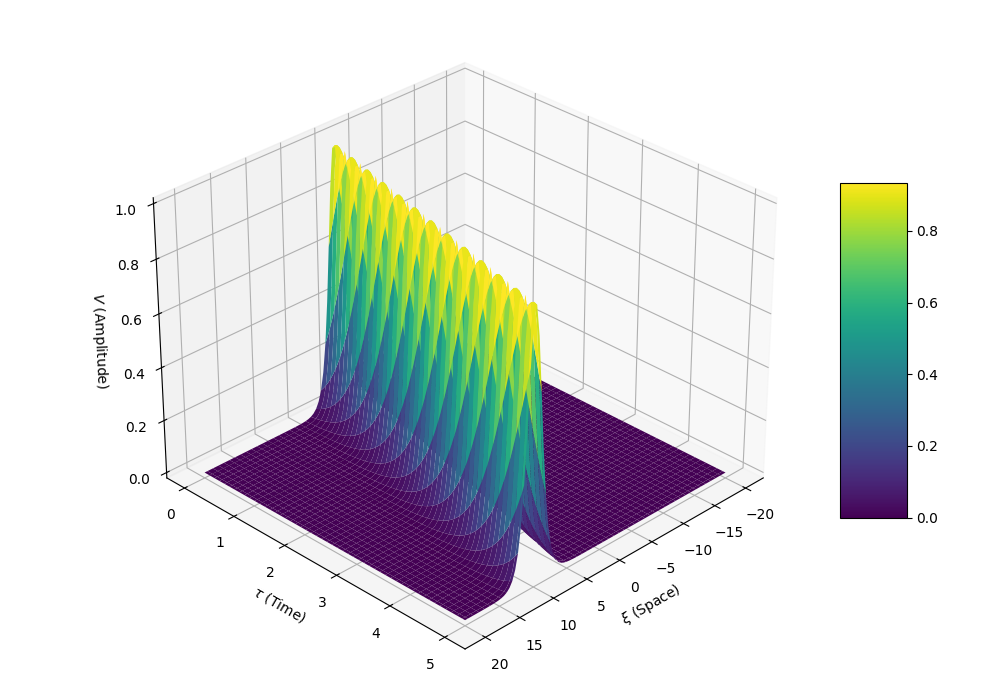
\includegraphics[width=0.6\textwidth]{solution_plot.png}
    \caption{バラクタダイオードで得られるソリトン解のプロット}
    \label{fig:soliton_lc}
\end{figure}


\section{おわりに}
次回以降は,このモデルをMLCCに適応できるように拡張する.

\subsection{参考文献}
\begin{itemize}
    \item 和達美樹 『岩波講座現代の物理学 非線形波動』 岩波書店 1992年
    \item pythonで学ぶ計算物理 ドキュメント » 5. 偏微分方程式 » 5.2. 【例題】KdV方程式\\ 
    \url{https://www.physics.okayama-u.ac.jp/~otsuki/lecture/CompPhys2/pde/kdv.html}\\
    (2025/11/20)
\end{itemize}

\newpage
\vfill
\end{multicols}

\end{document}
